%This is the fourth chapter of the dissertation

%The following command starts your chapter. If you want different titles used in your ToC and at the top of the page throughout the chapter, you can specify those values here. Since Columbia doesn't want extra information in the headers and footers, the "Top of Page Title" value won't actually appear.

\pagestyle{cu}
\graphicspath{{./Chapter4/images/}}

\chapter[Measuring the Low Energy Light and Charge Yield of Nuclear Recoils in Liquid Xenon][Measuring the Low Energy Light and Charge Yield of Nuclear Recoils in Liquid Xenon]{Measuring the Low Energy Light and Charge Yield of Nuclear Recoils in Liquid Xenon}
\label{chap:nerix}

%As was discussed in the second and third chapter of this work, understanding the response of liquid xenon to nuclear recoils is very important for the dark matter search as many candidates, including WIMPs, are expected to interact with atomic nuclei.  Liquid xenon detectors continue to grow in size yet this only makes their calibration, specifically with regards to nuclear recoils, increasingly difficult.  

As was discussed in the previous chapters, dual-phase liquid xenon TPCs lead the search for WIMPs.  These detectors continue to grow in size and reduce their background making them increasingly more sensitive to dark matter.  As mentioned in the previous chapter, XENON1T is the largest and most sensitive of these detectors with a total mass of 3,200 kg of liquid xenon \cite{aprile2017first}.  Since WIMPs are expected to interact primarily with atomic nuclei and the differential scattering rate of WIMPs and Standard Model particles are generally expected to increase with decreasing interaction energy, it is crucial to understand the properties of nuclear recoils in LXe down to the few keV energy scale.  

While larger detector sizes (in the form of larger fiducial volumes) make WIMP searches more and more sensitive, they do come with a drawback: calibrations, especially calibrations with external sources, becoming significantly more difficult.   However, understanding the signal output by a LXe TPC can essentially be broken down into two steps: the actual light and charge production and the detector physics.  While the detector physics is unique for each detector used and therefore must be measured for each one, the light and charge production mechanisms are only unique to the medium.  Therefore, if we can effectively decouple the two steps, we can measure the light and charge production mechanism in a detector optimized for calibrations and use it in other detectors.  

As LXe detectors have scaled in size, several of these optimized detectors have been built for exactly this purpose: to measure the light and charge production of liquid xenon to electronic and nuclear recoils.  While each of these detectors was slightly different and designed for a specific purpose, they shared the same relatively simple operating procedure: measure the light and charge produced from an interaction of a known type (electronic or nuclear recoil) and energy.  The neriX (Nuclear and Electronic Recoils in xenon) detector at Columbia University is one of these optimized detectors and has already successfully provided the most precise measurements of the light and charge yield of liquid xenon at multiple electric fields.  In this chapter, we will discuss the measurement of the light and charge yield of low energy nuclear recoils in liquid xenon using the neriX detector at Columbia University.

\section{Experimental Setup}

In chapter three, we discussed the nuclear recoil calibration of XENON1T.  In this calibration, an americium-beryllium (AmBe) source was used to irradiate the liquid xenon inside of the detector with MeV energy neutrons.  Simulation is performed to determine the energy spectrum of single scatters in the detectors but, for the most part, the spectrum is defined by the relative cross-section of elastic scatters at different energies ultimately resulting in an exponentially falling energy spectrum as seen in \figref{fig:xe1t_nr_energy_spec}.  In this calibration setup, the energy of each individual event is unknown and at the end of the day are using the entire energy spectrum to match our data.  While this can be an effective way to measure the response of liquid xenon to nuclear recoils, it proves to be very difficult in practice with such a featureless energy spectrum.  This type of measurement where one compares an energy spectrum to data is typically referred to as an \textit{indirect} measurement and has been used successfully to measure the light and charge production process of electronic and nuclear recoils \cite{aprile2013response, akerib2016tritium, aprile2017tritium}.

Measurements in neriX and other smaller, calibration optimized detectors follow a different approach.  A monoenergetic source is used to irradiate the detector where the incoming particle will scatter a single time before scattering into a secondary detector.  For electronic recoils, the secondary detector can be a high-purity germanium detector or sodium-iodide detector with an excellent energy resolution.  When this is the case, assuming the incoming radiation did not scatter with other materials around the detector, the energy of the interaction is known very precisely.  Unfortunately when measuring the response of liquid xenon to nuclear recoils in these detectors, no equivalent secondary detectors exist that will precisely measure the energy of the incoming neutron.  Instead we can use the position of the secondary detector as a proxy for the energy since the energy transferred to a xenon nucleus by a neutron is completely determined by the scattering angle.  This relationship between the energy of the recoiling nucleus and the angle is shown for non-relativistic neutron energies in \eqnref{eqn:nerix_energy_scattering_angle} where $m_n$ is the mass of the neutron, $m_{\textrm{Xe}}$ is the mass of the xenon nucleus, $E_r$ is the energy of the recoiling nucleus, $E_n$ is the energy of the incoming neutron, and $\theta$ is the scattering angle \cite{knoll2010radiation}.

\begin{equation}
        \label{eqn:nerix_energy_scattering_angle}
        E_r \approx E_n \frac{2 m_n m_{\textrm{Xe}}}{(m_n + m_{\textrm{Xe}})^2}(1 - \textrm{cos} \theta)
\end{equation}

A schematic of the experimental setup for neriX using this \textit{fixed-angle} technique is shown in \figref{fig:nerix_expt_schematic}.  The neutron source in this measurement was a \ce{^2H}$(d, n)$\ce{^3He} generator provided by the Schlumberger Princeton Technology Center which produces 2.45 MeV neutrons at an angle of $\frac{\pi}{2}$.  The secondary detectors used were Eljen Technologies M510 detectors filled with the EJ301 liquid scintillator, chosen for their excellent pulse shape discrimination.  


\begin{figure}[t]
        \centering
	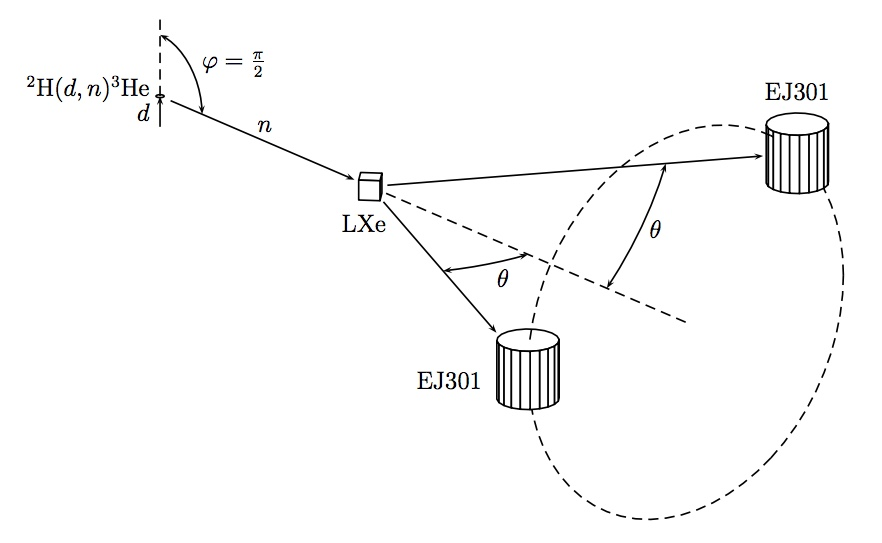
\includegraphics[width=0.9\textwidth]{nerix_expt_schematic}
	\caption{A schematic for the experimental setup used in this measurement of the light and charge yields for nuclear recoils.  .  Image Credit: \citeref{plante2011new}.}
	\label{fig:nerix_expt_schematic}
\end{figure}


\subsection{neriX Detector}

In this section we will discuss the neriX detector.  neriX was specifically designed to minimize the amount of inactive xenon and materials surrounding the TPC to minimize undetectable energy depositions and with electronics such that it can systematically scan electric fields ranging from approximately 0.15 V/cm to 2.5 kV/cm in the LXe.  These features make neriX an ideal detector for measuring the low-energy response of electronic and nuclear recoils at electric fields relevant to the dark matter search.

For more details on the design and construction of neriX, please refer to chapters four and five of \citeref{goetzke2015low}.

\subsubsection{TPC}

The neriX TPC (shown in \figref{fig:nerix_tpc_labeled}), like XENON1T, was also constructed with PTFE (teflon).  The teflon pieces in neriX are stackable and compressed by stainless steel springs.  The TPC at liquid xenon temperature has an inner diameter of 43 mm.  neriX also included four stainless steel hexagonal meshes and a single field shaping ring to control the electric fields inside of the TPC.  The cathode (used to produce the drift field inside the liquid xenon), the gate (kept at ground near the liquid surface), and the anode (used to extract electrons from the liquid surface and into the gas) were each made of  125 $\mu$m thick wires and 3 mm pitch (distance between parallel wire segments).  The final mesh was a screening mesh used to shield the bottom PMT and was also made a 3 mm pitch but with 25 $\mu$m thick wires (to reduce its surface area).  The field shaping ring is simply a copper coaxial wire embedded in the teflon wall of the TPC 7 mm above the cathode.  The location of the shaping ring was to maximize uniformity of the drift field at an electric field of 1 kV/cm.  The distance between the cathode and the gate mesh, the maximum drift distance of electrons in the TPC, was 23.4 mm.



\begin{figure}[t]
        \centering
	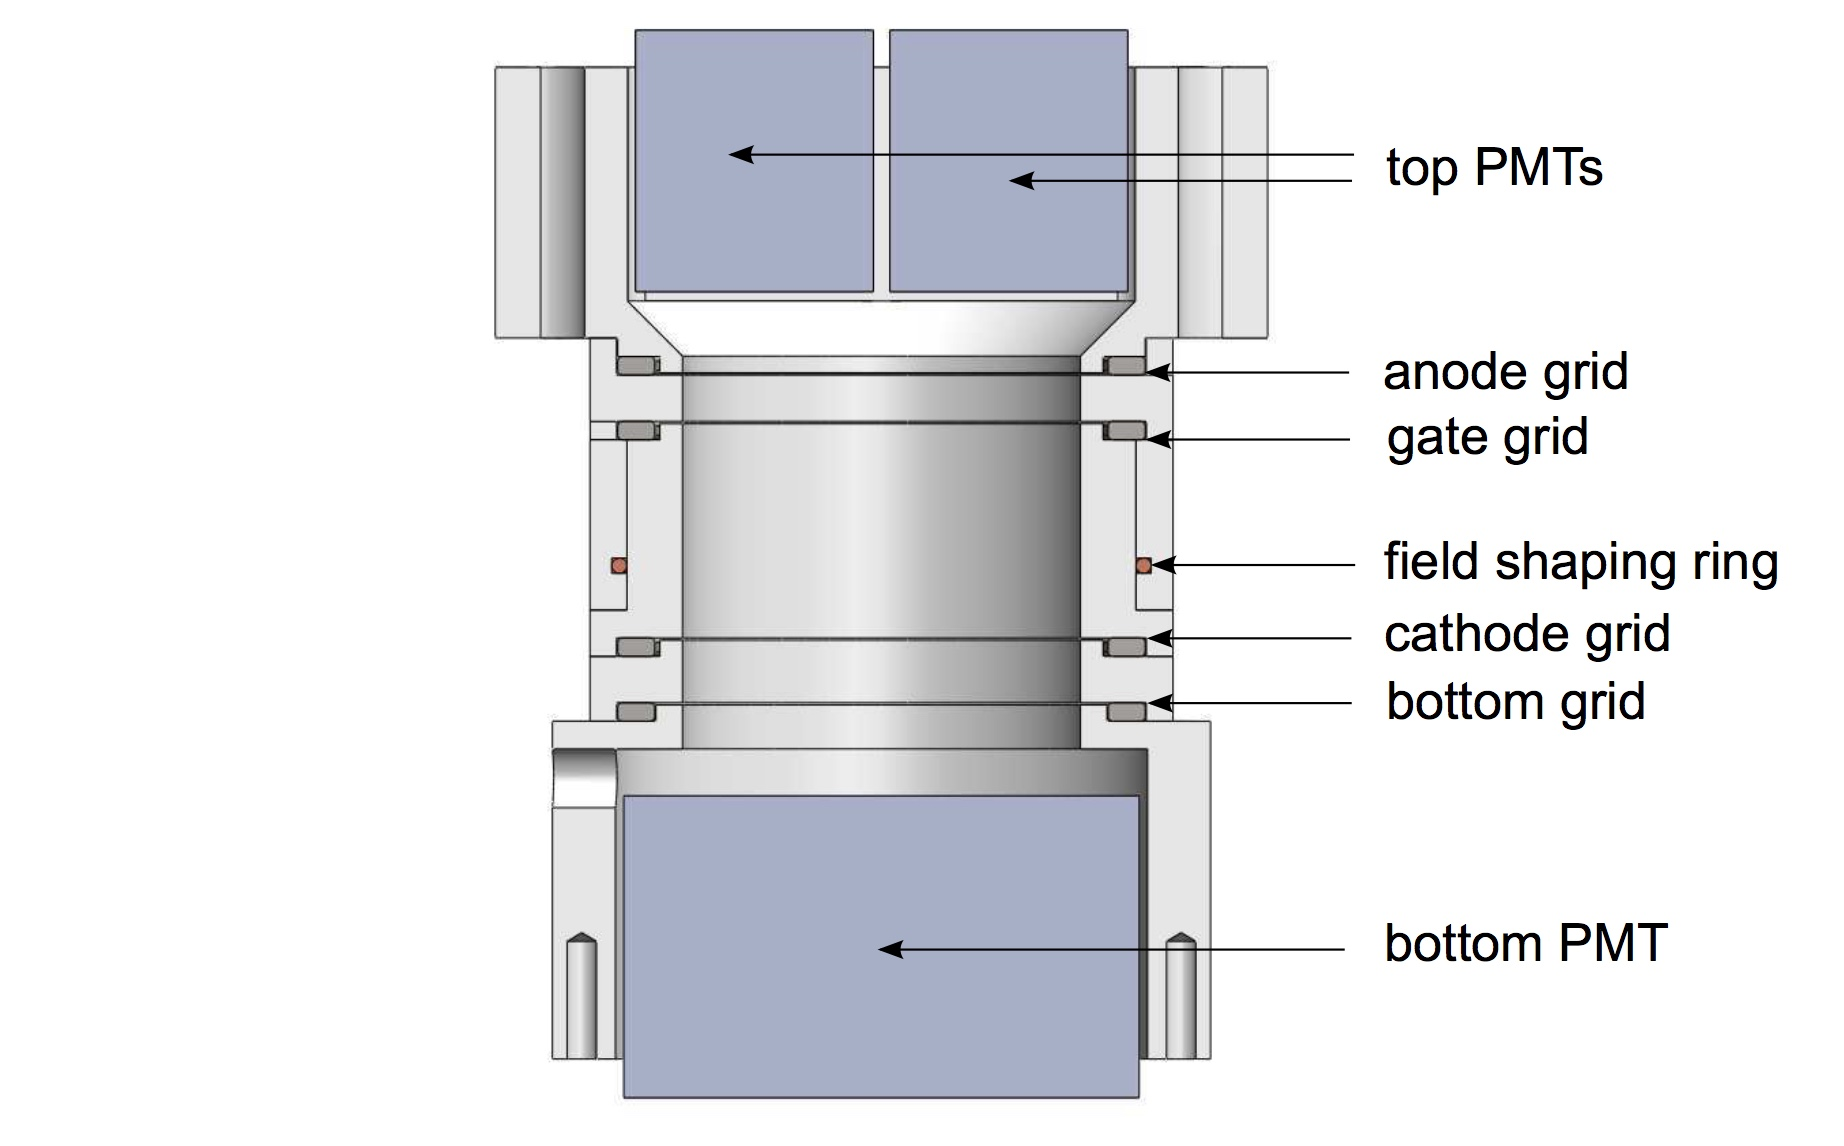
\includegraphics[width=0.8\textwidth]{nerix_tpc_labeled}
	\caption{The neriX TPC with meshes and PMTs shown.  The .}
	\label{fig:nerix_tpc_labeled}
\end{figure}
   

Six PMTs are installed in neriX: a single 2'' Hamamatsu R6041 PMT is installed below the screening mesh, four 1'' multianode Hamamatsu R8520-M4 PMTs are installed above the anode mesh, and a single 1'' Hamamatsu R8520-406 is installed in a light-tight stainless steel enclosure located above the TPC.  This final PMT is coupled to the TPC via a 1 mm fiber optic cable placed in between the four 1'' PMTs and is intended for measuring the decay times of singlet and triplet states in liquid xenon (although this measurement was not performed during the nuclear recoil calibration).  Since almost all light from the scintillation signal in the LXe is reflected at the liquid-gas interface, the bottom PMT is the only PMT used for measuring S1 and S2 signal size for simplicity leaving the top PMTs used for the position reconstruction of an interaction.

%The neriX TPC in many ways is very similar to the XENON1T TPC.  Both are made of PTFE (teflon), have meshes to produce



\subsection{Neutron Generator}


\begin{figure}[t]
        \centering
	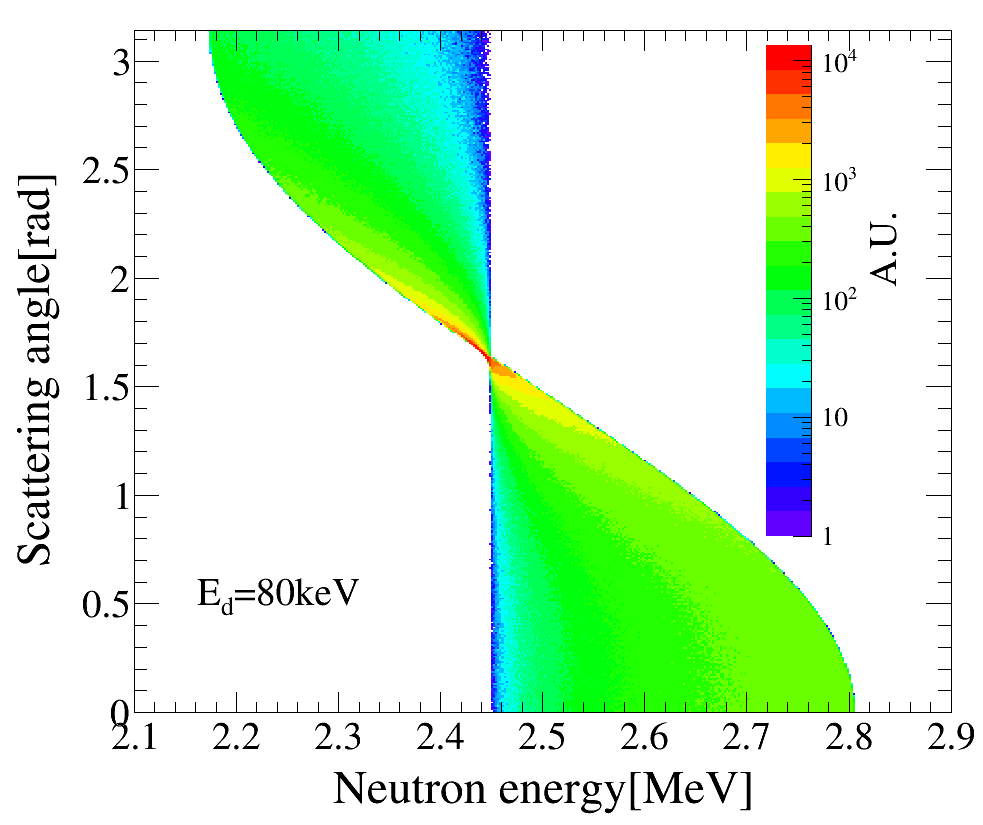
\includegraphics[width=0.75\textwidth]{nerix_minitron_angular_spec}
	\caption{.}
	\label{fig:nerix_minitron_angular_spec}
\end{figure}


\subsection{Liquid Scintillators}


In theory, any detector of ionizing radiation could act as the secondary detector in a nuclear recoil calibration.  In practice, however, the gamma ray background rate is large enough in a laboratory settings that detectors with high levels of discrimination are needed to differentiate neutrons from background in the secondary detector.  



\section{Characterization and Calibration of neriX}


\section{Nuclear Recoil Data Collection}


\section{Analysis of Nuclear Recoils in Liquid Xenon}


\section{Discussion}



